%
% This is the LaTeX template file for lecture notes for EE 382C/EE 361C.
%
% To familiarize yourself with this template, the body contains
% some examples of its use.  Look them over.  Then you can
% run LaTeX on this file.  After you have LaTeXed this file then
% you can look over the result either by printing it out with
% dvips or using xdvi.
%
% This template is based on the template for Prof. Sinclair's CS 270.

\documentclass[twoside]{article}
\usepackage{graphicx}
\usepackage{listings}
\lstset
{ %Formatting for code in appendix
    language=Matlab,
    basicstyle=\footnotesize,
    numbers=left,
    xleftmargin=1cm,
    stepnumber=1,
    showstringspaces=false,
    tabsize=1,
    breaklines=true,
    breakatwhitespace=false,
}

\graphicspath{ {images/} }
\setlength{\oddsidemargin}{0.25 in}
\setlength{\evensidemargin}{-0.25 in}
\setlength{\topmargin}{-0.6 in}
\setlength{\textwidth}{6.5 in}
\setlength{\textheight}{8.5 in}
\setlength{\headsep}{0.75 in}
\setlength{\parindent}{0 in}
\setlength{\parskip}{0.1 in}

%
% The following commands set up the lecnum (lecture number)
% counter and make various numbering schemes work relative
% to the lecture number.
%
\newcounter{lecnum}
\renewcommand{\thepage}{\thelecnum-\arabic{page}}
\renewcommand{\thesection}{\thelecnum.\arabic{section}}
\renewcommand{\theequation}{\thelecnum.\arabic{equation}}
\renewcommand{\thefigure}{\thelecnum.\arabic{figure}}
\renewcommand{\thetable}{\thelecnum.\arabic{table}}

%
% The following macro is used to generate the header.
%
\newcommand{\lecture}[4]{
   \pagestyle{myheadings}
   \thispagestyle{plain}
   \newpage
   \setcounter{lecnum}{#1}
   \setcounter{page}{1}
   \noindent
   \begin{center}
   \framebox{
      \vbox{\vspace{2mm}
    \hbox to 6.28in { {\bf EE 382V: Parallel Algorithms
                        \hfill Summer 2017} }
       \vspace{4mm}
       \hbox to 6.28in { {\Large \hfill Lecture #1: #2  \hfill} }
       \vspace{2mm}
       \hbox to 6.28in { {\it Lecturer: #3 \hfill Scribe: #4} }
      \vspace{2mm}}
   }
   \end{center}
   \markboth{Lecture #1: #2}{Lecture #1: #2}
   %{\bf Disclaimer}: {\it These notes have not been subjected to the
   %usual scrutiny reserved for formal publications.  They may be distributed
   %outside this class only with the permission of the Instructor.}
   \vspace*{4mm}
}

%
% Convention for citations is authors' initials followed by the year.
% For example, to cite a paper by Leighton and Maggs you would type
% \cite{LM89}, and to cite a paper by Strassen you would type \cite{S69}.
% (To avoid bibliography problems, for now we redefine the \cite command.)
% Also commands that create a suitable format for the reference list.
\renewcommand{\cite}[1]{[#1]}
\def\beginrefs{\begin{list}%
        {[\arabic{equation}]}{\usecounter{equation}
         \setlength{\leftmargin}{2.0truecm}\setlength{\labelsep}{0.4truecm}%
         \setlength{\labelwidth}{1.6truecm}}}
\def\endrefs{\end{list}}
\def\bibentry#1{\item[\hbox{[#1]}]}

%Use this command for a figure; it puts a figure in wherever you want it.
%usage: \fig{NUMBER}{SPACE-IN-INCHES}{CAPTION}
\newcommand{\fig}[3]{
			\vspace{#2}
			\begin{center}
			Figure \thelecnum.#1:~#3
			\end{center}
	}
% Use these for theorems, lemmas, proofs, etc.
\newtheorem{theorem}{Theorem}[lecnum]
\newtheorem{lemma}[theorem]{Lemma}
\newtheorem{proposition}[theorem]{Proposition}
\newtheorem{claim}[theorem]{Claim}
\newtheorem{corollary}[theorem]{Corollary}
\newtheorem{definition}[theorem]{Definition}
\newenvironment{proof}{{\bf Proof:}}{\hfill\rule{2mm}{2mm}}

% **** IF YOU WANT TO DEFINE ADDITIONAL MACROS FOR YOURSELF, PUT THEM HERE:

\begin{document}
%FILL IN THE RIGHT INFO.
%\lecture{**LECTURE-NUMBER**}{**DATE**}{**LECTURER**}{**SCRIBE**}
\lecture{8}{June 16}{Vijay Garg}{Andy Yang}
%\footnotetext{These notes are partially based on those of Nigel Mansell.}

% **** YOUR NOTES GO HERE:

% Some general latex examples and examples making use of the
% macros follow.  
%**** IN GENERAL, BE BRIEF. LONG SCRIBE NOTES, NO MATTER HOW WELL WRITTEN,
%**** ARE NEVER READ BY ANYBODY.
\section{Introduction}
In this section, we will be discussing sorting algorithms. Sorting can be separated into two categories: comparison-based, and non-comparison-based. Comparison-based algorithms use method such as $compare (A[i],A[j])$ where element at $i$ location is compared with element at $j$ location of the same array $A$. 

The following describes time complexity of insertion sort, quicksort, and mergesort.


\begin{center}
 \begin{tabular}{||c c c||} 
 \hline
      & worst-case time & average-case time \\ [0.5ex] 
 \hline\hline
 Insertion sort & $O(n^2)$ & $O(n^2)$ \\ 
 \hline
 Quicksort & $O(n^2)$ & $O({n \times \log(n))}$\\
 \hline
 Mergesort & $O({n \times \log(n))}$ & $O({n \times \log(n))}$ \\ [1ex] 
 \hline
\end{tabular}
\end{center}


Typically, quicksort is faster than mergesort. There are no comparison-based algorithms that can do better than $O({n \times \log(n))}$ time, which is the lower bound for both worst-case and average-case scenarios. 

If you have an unsorted array, the input to a sort has a permutation of $n!$. Each comparison eliminates half of the permutations. Therefore, the number of comparisons or the height of the tree would be $$height  \geq O(log(n!)) = O({n \times \log(n))}$$

For parallel algorithms, we can do a lot of comparison at a same time.

\section{Odd-even Sort}
Odd-even sort is sometimes called brick sort. The idea is compare elements in pairwise. During the first pass of the comparisons, the elements at odd indices are compared with their successors and are switched accordingly. During second pass of the comparisons, the elements at even indices are compared with their successors and are switched accordingly. Repeat the above process until after a set of odd and even comparisons, there are no more switching of elements in the array and is considered done. Notice that odd and even comparisons are considered as one step. It requires CRCW PRAM, but what we want is CREW or EREW. What if the smallest number in the array is at the most right side? We will run $n^2$ times, and be done. 

Given an unsorted array: \\
$3\hspace{0.5cm}11\hspace{0.5cm}2\hspace{0.5cm}9\hspace{0.5cm}6\hspace{0.5cm}1\hspace{0.5cm}5\hspace{0.5cm}8$

After odd entries comparisons: \\
$3\hspace{0.5cm}11\hspace{0.5cm}2\hspace{0.5cm}9\hspace{0.5cm}1\hspace{0.5cm}6\hspace{0.5cm}5\hspace{0.5cm}8$

After even entries comparisons: \\
$3\hspace{0.5cm}2\hspace{0.5cm}11\hspace{0.5cm}1\hspace{0.5cm}9\hspace{0.5cm}5\hspace{0.5cm}6\hspace{0.5cm}8$

After odd entries comparisons: \\
$2\hspace{0.5cm}3\hspace{0.5cm}1\hspace{0.5cm}11\hspace{0.5cm}5\hspace{0.5cm}9\hspace{0.5cm}6\hspace{0.5cm}8$

After even entries comparisons: \\
$2\hspace{0.5cm}1\hspace{0.5cm}3\hspace{0.5cm}5\hspace{0.5cm}11\hspace{0.5cm}6\hspace{0.5cm}9\hspace{0.5cm}8$

\ldots

\begin{center}
 \begin{tabular}{||c c c||} 
 \hline
      & Time & Work \\ [0.5ex] 
 \hline\hline
 Odd-even sort & $O(n)$ & $O(n^2)$ \\ 
 [1ex] 
 \hline
\end{tabular}
\end{center}



\subsection{Oblivious Sorting Algorithm}

Oblivious sorting algorithm makes the exact same comparisons. The same entries in the array will be compared irrespective of the actual entries. Have a comparitor takes two inputs $x$, $y$, and generates $max(x,y)$ and $min(x,y)$. Even the entries are sorted, they still need to go through the comparitors.

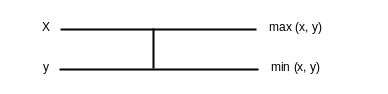
\includegraphics[scale=0.5]{g1}

Odd-even sort is an oblivious sorting algorithm. It can be represented graphically as below:

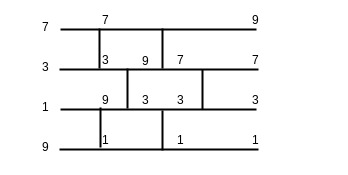
\includegraphics[scale=0.5]{g2}

Time is corresponding to the depth of the circuit, or length of the wall.
Work is corresponding to the number of comparitors.

\section{Bitonic Sort (Batcher Sort)}
In mergesort, we divide the array into two parts, and sort them individually and merge, but merging is not easy. Instead of sorting them in the same direction, bitonic sort sorts them one in ascending direction and the other in descending direction, and sort them recursively. The first half would be in ascending order, and the second half would be in descending order.

Mergesort sorts sequentially merge one things at a time, but we want to compare multiple elements at the time.

We will do left bitonic sort, right bitonic sort, and do bitonic merge. The bigger element go up, and the smaller element go down. We would have upper and lower part, and the upper part is all bigger than elements in the lower part. 

In $O(logn)$ step, we will be done since we recursively divide up the array. 

\subsection{Bitonic Sequence}
Monotonic sequence is either in descreasing order or increasing order. Bitonic sequence is either first part is increasing and the second part is descreasing or the first part is descreasing and the second part is increasing. The following shows graphical representation of the bitonic sequence and its element comparisons. 

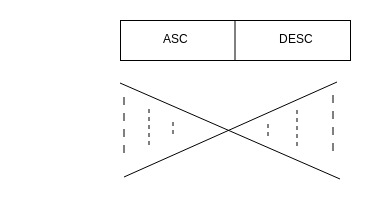
\includegraphics[scale=0.5]{g3}

Think of bitonic sequence as two separate arrays. Given a bitonic sequence $A$, where $h$ indicates the location of the largest element and $lo$ indicates the location of the smallest element. 

$\hspace{0.5cm}\hspace{0.5cm}\hspace{1cm}h\hspace{0.5cm}\hspace{0.65cm}lo\hspace{0.5cm}\hspace{0.5cm}$

$3\hspace{0.5cm}4\hspace{0.5cm}5\hspace{0.5cm}7\hspace{0.5cm}6\hspace{0.5cm}1\hspace{0.5cm}2\hspace{0.5cm}$

There exist two monotonic sequences $A[h..lo]$ and $A[lo..h]$ with the second array rotating to get the bitonic sequence. 

\textbf{Definition:} A sequence $A[0]...A[n-1]$ is bitonic if there exist two indices $l$ and $h$ such that $A[l..h]$ is an ascending sequence and $A[h..l]$ is descending sequence. 

\subsection{Zero-one Principle}
\textbf{Theorem:} If a comparator network correctly sorts all sequences $0$ and $1$, then it correctly sorts all integer sequences. 

Proof: By contradiction, if a comparator network correctly sorts all $0-1$ sequence but did not correctly sort some of the integer sequence. 

Bitonic $0-1$ sequences are shown as the follows, given that $j,k,l\geq 0$

$0^j\hspace{0.5cm}1^k\hspace{0.5cm}0^l$\\

$1^j\hspace{0.5cm}0^k\hspace{0.5cm}1^l$

\subsection{Monotonic Function}
A monotonic function is a function that preserves the concept of order such as $3\leq5$. Instead of using $x_1$ as input, apply $f(x_1)$, the resulting ordering would be same as if input were $x_1$. 

A function is monotonic iff $x\leq y -> f(x)\leq f(y)$.

\begin{center}
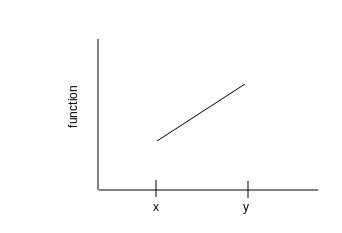
\includegraphics[scale=0.5]{g5}
\end{center}

$f(x) = -6x$ would not be monotonic, whereas $f(x) = 6x$ would be a monotonic function.

\textbf{Claim:} Given a function $f(x): x->x$ is monotonic, it preserves miniumum and maximum operator. 
$$f(min(x,y)) = min(f(x),f(y))$$
$$f(max(x,y)) = max(f(x),f(y))$$

\begin{center}
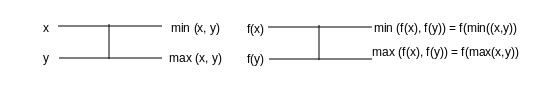
\includegraphics[scale=0.5]{g6}
\end{center}

Instead of give $x$,$y$ as the inputs, give $f(x)$, $f(y)$.

Suppose for all $x_1..x_n$ such that the network does not sort it correctly, the result would be that for all $x_i$,$x_j: x_i < x_j$, the output puts $x_j$ before $x_i$ or output is faulty.

\subsection{Bitonic Merge Lemma}
Bitonic merge lemma states that given a bitonic sequence $A$ of length $2n$. Let

$B = min(A[i],A[i+n]) |  0 \leq i < n$\\
$C = max(A[i],A[i+n]) |  0 \leq i < n$

Then $B$ and $C$ are both bitonic and all values in $B$ are less than or equal to all values in $C$. 

Let $A = 2\hspace{0.5cm}9\hspace{0.5cm}11\hspace{0.5cm}16\hspace{0.5cm}14\hspace{0.5cm}12\hspace{0.5cm}2\hspace{0.5cm}1\hspace{0.5cm}$\\

$B = min(2,14),min(9,12),min(11,2),min(16,1)$\\

$C = max(2,14),max(9,12),max(11,2),max(16,1)$\\

$B=[2,9,2,1]$, which is bitonic \\
$C=[14,12,11,16]$, which is bitonic

Case analysis of using 0-1 sequence can be used to verify the correctness of bitonic merge lemma. 


\subsection{Bitonic Sort Algorithm}

Bitonic sort recursively divide the array into two halves, and in each bitonic sort function call bitonicMerge to recursively sort the first half in ascending order, and sort the second half in descending order. Each bitonicMerge call would result in a bitonic sequence, which allows bitonic merge at a higher call level to recursively breaks the bitonic sequence into two halves and compares the elements and swap when necessary. The algorithm implementations are shown below:

\begin{lstlisting}
void bitonicSort (int lo, int n, boolean dir) <- n is power of 2
	if (n>1) {
		int m = n/2
		bitonicSort (lo, m, ASC)
		||
		bitonicSort (lo+m, m, DESC)
		bitonicMerge (lo, n, dir)
	}
}

void bitonicMerge (int lo, int n, boolean dir){
	if (n>1) {
		int m = n/2;
		for (int i = lo; i < lo + m; i++) in parallel do 
			compare (i, i + m, dir);//minimum on one side, maximum on the other side, double recursion
			bitonicMerge(lo, m, dir)
			||
			bitonicMerge(lo+m, m, dir)
	}
}

//Assume i < j, guaranteed by the caller
void compare (int i, int j, boolean dir) {
	if (dir == (a[i] > a[j] {
		exchange (i,j);
	}
}
\end{lstlisting}

The followings are graphical representation of bitonic sort algorithms for four inputs and eight inputs respectively.

\begin{center}
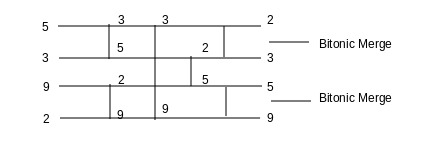
\includegraphics[scale=0.5]{g7}\\
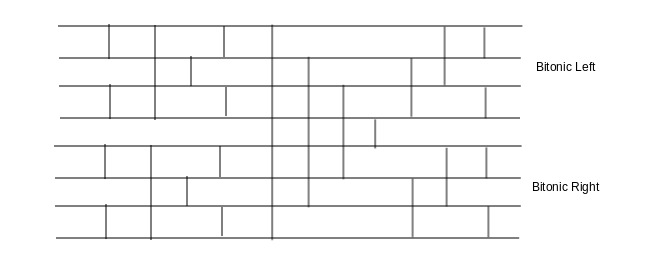
\includegraphics[scale=0.5]{g8}
\end{center}

\subsection{Bitonic Sort Complexity Analysis}

Bitonic sort: $T(n) = T(n/2) + O(logn)$ (bitonic merge)\\
$T(1)=O(1);$\\
$T(n)=logn + (logn - 1) + (logn - 2) + ... $ (at each level)\\
$T(n)=O(logn)^2$

$W(n) = O(n \times log^2n)$

There exists AKS network that runs $O(logn)$ and has work $O(n\times logn)$,but it is not fast enough to bitonic sort. 

\end{document}







